\chapter{Existing Techniques and Models}
\label{chap:current_models}

In this study we aim to improve on existing speech feature extraction using a trained vision CNN.
In order to understand this process, we first need to understand the feature extraction techniques as well as how CNNs work.
This chapter provides an overview of each speech feature extraction technique, namely spectrograms, filterbanks and MFCCs, and the convolution process within CNNs. 
Thereafter it looks specifically at the inner structure of the VGG16 vision network.

\section{Speech Features}

For the task of speech recognition, generic time domain sound waves are an ineffective choice for input data. 
They are large files that would cause the resultant machine learning model to have to accept massively large input sizes. 
For this reason, the sound waves are often converted to the frequency domain into spectrograms. 

Spectrograms contain all the useful information about the speech data in a far more concise format, but can sometimes still be fairly large data structures. 
Therefore, spectrograms are usually further reduced to filterbanks and MFCCs, which more accurately reflect the way humans perceive audio information and reduce the input dimension size.

\subsection{Spectrograms}

Speech data is often very inefficient to work with in the time domain, therefore, discrete time domain signals are often converted to the frequency domain via a process called Discrete Fourier Transform (DFT). 
The DFT ($H[k]$) of a discrete time domain signal ($h[n]$) is calculated by first windowing the signal using the Hamming Window ($w[n]$) with window size $N$ to obtain $h_{w}[t]$:
\begin{gather}
    w[n] = 0.54+0.46\cos\Big(\frac{\pi n}{N-1}\Big), \quad 0 \leq n \leq N-1 \\
    h_{w}[n] = h_{s}[n] \cdot w[n]
\end{gather}

Thereafter, the signal must be made periodic in time in order to discretise the frequency domain signal. 
This is done by convolving the signal with the periodic impulse function in $N$ to obtain $h_{p}[n]$:

\begin{equation}
    h_{p}[n] = h_{w}[n] \ast \delta(n-kN), \quad k=(0,1,\dotsc,N-1)
\end{equation}

The Fourier Transform (FT) of $h_{p}[n]$ then forms our desired DFT function:

\begin{equation}
    H[k] = \mathcal{F} \{ h_{p}[n] \}
\end{equation}

In summary, this process can be written as follows:

\begin{equation}
    H[k] = \mathtt{DFT} \{ h_{p}[n] \} = \displaystyle\sum_{n=0}^{N-1} h[n] \cdot e^{\displaystyle\frac{-j2\pi kn}{N}}
\end{equation}

The problem with simply calculating the DFT of speech data, is that speech is a non-stationary signal, Thus the DFT will calculate each frequency present throughout the entire word. 
Therefore, spectrograms are obtained by performing the Short Time Fourier Transform (STFT) on the speech sound wave. 

STFT works by segmenting the sound wave into frames of length $N$ seconds, sampled every $R$ seconds, and then calculating the log power of the DFT for each individual frame and concatenating the two-dimensional functions into a three-dimensional surface. 
The third dimension is then converted to colour, forming a spectrogram of the sound signal. 
This process is visualised in Figure~\ref{fig:spec_example} for the function $h[t]=\sin\big(2\pi f_{w_1} t + 100 \cdot \cos(2\pi f_{w_2} t) \big)$, with $f_{w_1}= 8 \mathrm{kHz}$, $f_{w_2}= 4 \mathrm{Hz}$.
The power of the DFT can be calculated as follows:

\begin{equation}
    P = \log\bigg(\frac{|\mathtt{DFT}(x_i)|^2}{N}\bigg)
\end{equation}

It is important to note that, computationally, the DFT is calculated by means of the Fast Fourier Transform (FFT) function, which gives the exact same results, but exploits the symmetries and periodicity of the DFT to save on computation. 
The FFT changes the DFT from an $O(N^2)$ computation to $O(N)$.

\begin{figure}[ht]
    \centering
    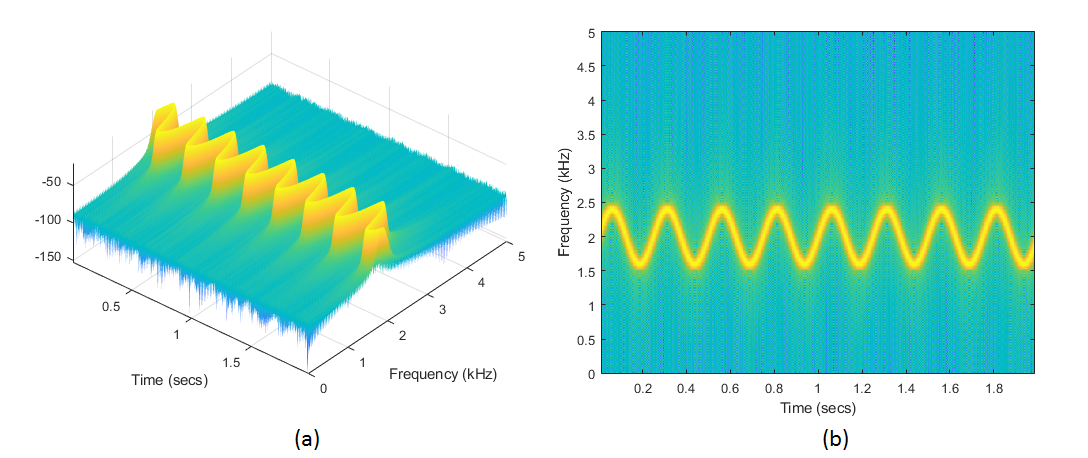
\includegraphics[width=0.9\linewidth]{content/fig/spec_example.png}
    \caption{
    (a) The STFT of a function with varying frequency and, 
    (b) The STFT in (a) visualised as a spectrogram.
    }
    \label{fig:spec_example}
\end{figure}

\subsection{Filterbanks}

Spectrograms are a useful feature for analysing frequency characteristics of a signal, but when it comes to speech in particular, they still contain a lot of unnecessary information. 
Human speech, for instance, falls mainly within 80 Hz and 8 kHz, thus removing the need for very high frequency capturing. 
Even more, the human ear does not distinguish different levels of frequencies equally. 
We are able to distinguish the difference between an 80 Hz signal and a 100 Hz signal far greater than between 3 kHz and 3.1 kHz.

It is this property that gives rise to the Mel-scale. 
The Mel-scale aims to mimic the non-linear human ear perception of sound by being more discriminative at lower frequencies and less discriminative at higher frequencies. 
We can convert between Hertz ($f$) and Mel ($m$) using the following equations \cite{fayek_2016}:

\begin{equation}
    m = 2595 \log_{10} (1 + \frac{f}{700})
\end{equation}

\begin{equation}
    f = 700 (10^{m/2595} - 1)
\end{equation}

Filterbanks are calculated by applying triangular filters (usually 40), spaced according to the Mel-scale as shown in Figure~\ref{fig:mel_filters}, over the speech spectrogram. 
This results in a $40\times N$ array, where $N = \frac{\mathrm{time}}{f_s}$, which is a quarter the size of the previous spectrograms.
These triangular filters can be modelled by the following function:

\begin{equation}
    H_m(k) =
  \begin{cases}
      \hfil 0 & k < f(m - 1) \\
      \dfrac{k - f(m - 1)}{f(m) - f(m - 1)} & f(m - 1) \leq k < f(m) \\
      \hfil {1} & k = f(m) \\
      \dfrac{f(m + 1) - k}{f(m + 1) - f(m)} & f(m) < k \leq f(m + 1) \\
      \hfil {0} & k > f(m - 1) \\
  \end{cases}
\end{equation}

\begin{figure}[ht]
    \centering
    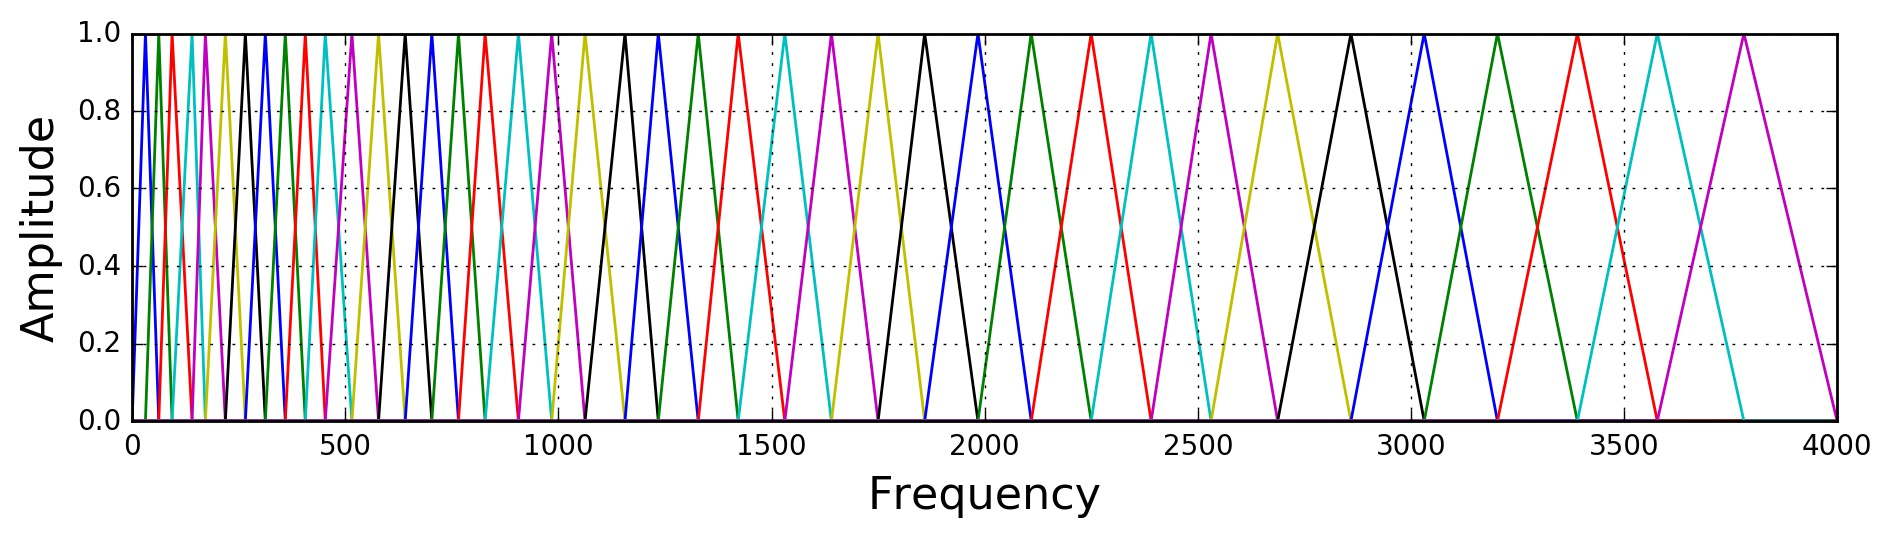
\includegraphics[width=0.9\linewidth]{content/fig/mel_filters.jpg}
    \caption{40 filterbanks on the Mel-scale.\cite{fayek_2016}}
    \label{fig:mel_filters}
\end{figure}

\subsection{Mel-Frequency Cepstral Coefficients (MFCCs)}

Going one step further from filterbanks, mel-frequency cepstral coefficients aim to tackle the highly correlated nature between each filterbank. 
This correlated nature of the filterbanks is because, as can be seen by Figure~\ref{fig:mel_filters}, each filter overlaps with the filters next to it.

To understand how MFCCs aim to tackle this problem, it helps to look at filterbanks as a continuous time signal instead of a discrete frequency spectrum.
The overlapping nature of the filters would then cause small peaks within the resulting signal, which can be viewed as high frequency noise on top of the desired signal.

Usually, when we want to remove high frequency noise from a signal, we calculate the FT to transform the signal to the spectral (frequency) domain, then simply remove the higher frequencies. 
When calculating the FT of a spectral signal, it is called moving to the cepstral domain, and thus the name, mel-frequency cepstral coefficients.

Instead of calculating the FT of the filterbanks, however, MFCCs are calculated by using the Discrete Cosine Transform (DCT).
The DCT gives a fairly similar result as the DFT, and can be expressed as follows:

\begin{equation}
    X[k] = \mathtt{DCT} \{ x[n] \} = \displaystyle\sum_{n=0}^{N-1} h[n] \cdot \cos\bigg(\displaystyle\frac{\pi}{N}\Big(n+\frac{1}{2}\Big)k\bigg)
\end{equation}

After the DCT of the filterbanks are calculated, only twelve of the 26 DCT coefficients are kept, removing fast changes in the filterbanks and effectively applying a cepstral low-pass filter (LPF) on them. 
The energy of each frame is also appended to the bottom of the MFCC to result in a 13 data points per frame array.

There often lies valuable information in the trajectories of MFCC coefficients over time, but the MFCC feature vector only describes the spectral envelope of a single frame.
Therefore, it is common to append the differential (delta) and acceleration (delta-delta) coefficients of the MFCC to the feature vector. 
The delta coefficients are calculated with the following formula:

\begin{equation}
    d_t=\displaystyle\frac{\sum_{n=0}^{N-1} n(c_{t+n}-c_{t-n})}{2\sum_{n=0}^{N-1} n^2}
\end{equation}
where $d_t$ is the delta coefficient and $c_t$ the filterbank value of frame $t$.
$N$ is commonly set to two. 
The delta-delta coefficients are calculated similarly, except the MFCC values are substituted by the delta coefficients.

Applying all this results in a $39\times N$ array, where $N = \frac{\mathrm{time}}{f_s}$, thus a slightly smaller feature vector than filterbanks, yet containing more effective information about the speech data.

\section{Convolutional Neural Networks (CNNs)}

In this study we hope to improve upon existing speech feature extraction techniques by using the learned features from image classification CNNs. 
In order to understand how CNNs extract features from images, and automatically learn how to extract the most relevant features, we must first look in to how they work.

\subsection{Convolution}

The main aspect of a CNN is the actual convolutional layers. 
Each layer, as the name suggests, convolves the input it is given with one or multiple filter kernels.
Discrete convolution for one element of an input feature $I$ with a $N \times M$ filter kernel $K$ can be defined as follows:

\begin{equation}
    (I \ast K)[i, j] = \displaystyle\sum_{m=0}^{M-1}\displaystyle\sum_{n=0}^{N-1}I[m,n] K[i-m, j-n]
\end{equation}

Performing this operation for every combination of $i$ and $j$ results in a feature map that in essence describes how prominently the feature $K$ appears at each point within $I$.

In practice, CNNs don't actually compute the convolution between two filters, but instead the cross-correlation \cite{murray_2018}. 
Since commutativity is not important for most CNNs, it avoids the need of having to flip one of the signals. 
Cross-correlation is very similar to convolution and will be used interchangeably throughout the text.
It can be defined as follows:

\begin{equation}
    (I \ast K)[i, j] = \displaystyle\sum_{m=0}^{M-1}\displaystyle\sum_{n=0}^{N-1}I[m,n] K[i+m, j+n]
\end{equation}

When given an input feature of size $I \times J$, convolved with a filter kernel of $3\times3$, the resultant feature map will be of size $(I-2)\times(J-2)$.
To avoid this, the input feature is often zero padded on each edge with one zero to form an input of size $(I+2)\times(J+2)$, keeping the feature map the same size as the original input.

In neural networks, the act of convolution can be seen as a sparsely connected neural layer. 
Each weight ($h_i$) is connected to a limited amount of input neurons ($x_i$) from the previous layer.
The weight then performs a linear transformation on the input neurons. 
For a one dimensional input and a connection level of three, this process is visualised in Figure~\ref{fig:cnn_layer}, and can be described as follows:

\begin{equation}
    h_i = \displaystyle\sum_{j=-1}^{1}w_{j}x_{i+j}+b_i
\end{equation}

\begin{figure}[ht]
    \centering
    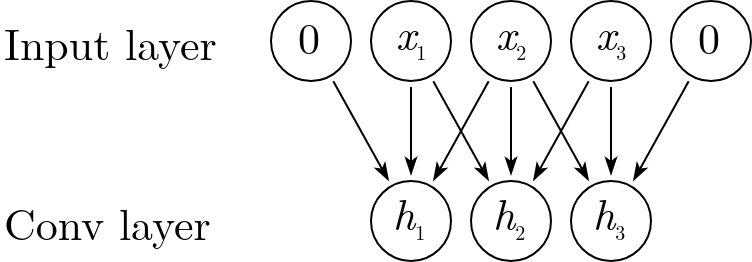
\includegraphics[width=0.5\linewidth]{content/fig/cnn_layer.png}
    \caption{Visualisation of a single convolutional layer.}
    \label{fig:cnn_layer}
\end{figure}

The formula for obtaining the weight is thus equivalent to convolution, with the added benefit of adding a bias $b$ to the final filter result. 

It should also be mentioned that most CNN layers also consist of a ReLU layer, which simply applies an activation function of $f(x)=\mathrm{max}(0,x)$ to the output of the convolutional layer. 
This increases the nonlinear properties of the decision function without affecting the receptive field \cite{pmlr-v15-glorot11a}.

In order to reduce the dimensionality of the feature maps, convolutional neural networks make use of max pooling.
Max pooling simply applies an $N \times N$ filter across its input, outputting only the maximum value within the filter.
The filter is then passed through the entire input, usually with a stride of $N$, reducing the each input dimension by a factor of $N$.

\subsection{VGG16}

The VGG16 CNN, first proposed by Simonyan et al. \cite{DBLP:journals/corr/SimonyanZ14a}, achieved an image classification accuracy of 92.7\% on the ImageNet database, a data set of more than 14 million images belonging to 1\,000 different classes, in 2014 \cite{ILSVRC15}.
To achieve this accuracy, it employs 13 convolutional layers in total, with four max pooling layers in-between to reduce dimensionality.
The full structure can be seen in Figure~\ref{fig:vgg16}.

\begin{figure}[ht]
    \centering
    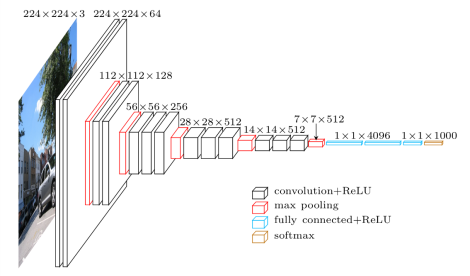
\includegraphics[width=0.6\linewidth]{content/fig/vgg16.png}
    \caption{Macro architecture of VGG16 network. \cite{leonardblier_2016}}
    \label{fig:vgg16}
\end{figure}

The VGG16 network makes use of $3\times3\times N$ sized filter kernels, with $N$ being the number of feature maps in the previous layer, with a stride of one and a padding of one to keep the feature map the same dimensionality as the input.
Max pooling is performed by a $2\times2$ window with a stride of two, effectively halving the first two dimensions of the input \cite{DBLP:journals/corr/SimonyanZ14a}.

For this study, a TensorFlow adaptation of the VGG16 network was used\cite{frossard_2016}.
This model was further adapted to be able to accept differently sized images and added functionality to retrieve the output of each convolutional layer was written.

It should be noted how efficient CNNs can be in extracting features from images.
Where it may seem obvious for humans to design a filter kernel that might detect edges, a CNN can result in kernels that are much less straightforward, but result in far more useful features.
A simple example within the VGG16 network is shown in Figure~\ref{fig:filter_36}, keeping in mind that the first layer of filters are of size $3\times3\times3$, and that the third dimension is displayed as RGB colours.
This shows that a small filter kernel in the first layer of the CNN can already be used to capture features as complex as eyes.

\begin{figure}
    \centering
    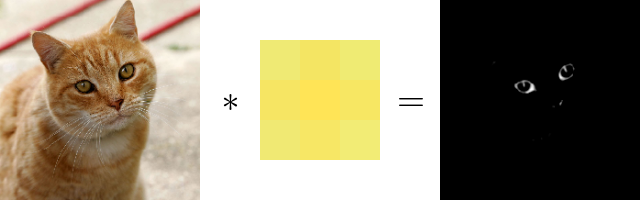
\includegraphics[width=0.6\linewidth]{content/fig/kernel36.png}
    \caption{Example input and output from  kernel 36 of the first convolutional layer in the VGG16 network.}
    \label{fig:filter_36}
\end{figure}

A full list of the first layer of filter kernels can be found in Appendix~\ref{appen:conv1_1}.
Going further down the layers produces even more ambiguous feature maps. 


The ambiguity and general nature of these filter kernels and the feature maps they generate form the basis for employing them as feature extraction techniques for different types of data, such as speech.